\documentclass[14pt,a4paper]{extreport}

% ---------------------------------------------------------------------------
% Packages
% ---------------------------------------------------------------------------
\usepackage[margin=1in]{geometry}
\usepackage{graphicx}
\usepackage{amsmath,amssymb}
\usepackage{enumitem}
\usepackage{fancyhdr}
\usepackage{titlesec}
\usepackage{xcolor}
\usepackage{booktabs}
\usepackage{longtable}
\usepackage{array}
\usepackage{float}
\usepackage[hidelinks]{hyperref}
\usepackage{etoolbox}

% ---------------------------------------------------------------------------
% TODO (fill these in before compiling / submitting):
%   - Screenshots / figures for each dashboard page
% ---------------------------------------------------------------------------
\newcommand{\groupnumber}{07}

% ---------------------------------------------------------------------------
% Header / footer
% ---------------------------------------------------------------------------
\pagestyle{fancy}
\fancyhf{}
\fancyhead[L]{CS661 Project Report}
\fancyhead[R]{Group \groupnumber}
\fancyfoot[C]{\thepage}
\renewcommand{\headrulewidth}{0.4pt}

% Smaller heading sizes throughout (chapter/section/subsection/subsubsection).
\titleformat{\chapter}[hang]{\normalfont\Large\bfseries}{\thechapter}{1em}{}
\titlespacing*{\chapter}{0pt}{0pt}{20pt}
\titleformat{\section}{\normalfont\large\bfseries}{\thesection}{1em}{}
\titleformat{\subsection}{\normalfont\normalsize\bfseries}{\thesubsection}{1em}{}
\titleformat{\subsubsection}{\normalfont\normalsize\itshape}{\thesubsubsection}{1em}{}

% Chapters no longer force a page break, so short chapters (e.g. Project
% Repository) don't leave the rest of the page blank.
\makeatletter
\patchcmd{\chapter}{\if@openright\cleardoublepage\else\clearpage\fi}{}{}{}
\makeatother

\setcounter{secnumdepth}{4}
\setcounter{tocdepth}{4}

\begin{document}

% ===========================================================================
% Title Page
% ===========================================================================
\begin{titlepage}
    \centering
    \vspace*{2cm}

    {\Large \bfseries NIFTY-50 Visual Analytics: Exploring Two Decades of \\[2mm]
    Indian Stock Market Behaviour Through Interactive Dashboards \par}

    \vspace{1.5cm}
    {\large Group \groupnumber \par}

    \vspace{0.5cm}
    {\normalsize
    Abhay Kesarwani (240026) \\
    Sayani Patra (230943) \\
    Rishit Bhutra (210857) \\
    Deepak (240327) \\
    Navin Patel (240685) \\
    Nitish (240710) \\
    Riddhima Verma (240865) \\
    Gaikwad Shivam Pradeep (240391)
    \par}

    \vspace{1.5cm}
    {\normalsize CS661 -- Big Data Visual Analytics \par}
    {\normalsize Department of Computer Science and Engineering \par}
    {\normalsize Indian Institute of Technology Kanpur \par}
\end{titlepage}

\tableofcontents

% ===========================================================================
\chapter{Project Repository}
% ===========================================================================

The complete codebase, Dash application, data pipeline, and documentation for
this project are available on GitHub:

\begin{center}
    \url{https://github.com/navinp24/CS661_project}
\end{center}

% ===========================================================================
\chapter{Introduction}
% ===========================================================================

Financial markets generate vast volumes of high-frequency, multi-dimensional
data every trading day -- prices, volumes, turnover, and delivery statistics
across hundreds of listed companies. Making sense of this data requires more
than raw numbers: it requires visual analytics techniques that can reveal
correlations, risk structures, systemic shocks, sector rotations, and
long-term growth patterns that are otherwise invisible in tabular form.

This project investigates two decades (2000--2021) of historical daily
trading data for the \textbf{NIFTY-50}, the benchmark stock market index of
the National Stock Exchange of India (NSE), covering 49 of its 50
constituent companies across 13 sectors. Through a suite of interactive,
linked visual analytics dashboards, we explore multiple dimensions of market
behaviour -- including inter-stock correlation structure, risk-return
clustering, market-wide shocks and anomalies, sector rotation dynamics, and
sector-level growth attribution.

Our aim is to present clear, interactive, and insightful visual narratives
that are accessible to both technical and non-technical stakeholders --
analysts, retail investors, and researchers alike. By combining a
reproducible data-cleaning pipeline, an embedded analytical database, and
Python-based interactive visualization tooling (Dash and Plotly), this
project seeks to demonstrate how big-data visual analytics techniques can be
applied end-to-end, from raw CSV files to production-style interactive
dashboards.

% ===========================================================================
\chapter{Objective}
% ===========================================================================

The primary objective of this project is to design, build, and analyze a
multi-page interactive visual analytics system for exploring NIFTY-50 stock
market behaviour over a 21-year period. Specifically, the project aims to:

\begin{itemize}
    \item Build a reproducible data pipeline that ingests raw per-company
        trading CSVs, merges them with sector metadata, cleans and validates
        the data, and loads it into an efficient query engine.
    \item Identify clusters of stocks that move together using correlation
        analysis and hierarchical clustering, to understand systemic
        co-movement risk.
    \item Characterize each stock's risk-return profile and group companies
        into behaviourally similar clusters using unsupervised learning.
    \item Detect market-wide shocks (crashes and rallies) and quantify their
        severity and sector-level dispersion using rolling statistical
        anomaly detection.
    \item Visualize sector rotation -- how capital flows between leading,
        weakening, lagging, and improving sectors over time relative to the
        broader market.
    \item Attribute long-term growth (CAGR) to individual companies and
        sectors, and present this hierarchy interactively.
    \item Present all insights through an intuitive, filterable, and
        cross-linked dashboard built with Dash, Plotly, and an embedded
        DuckDB analytical database.
\end{itemize}

These objectives are designed to facilitate a deeper understanding of market
structure, systemic risk, and sector dynamics in one of the world's fastest
growing major stock markets.

% ===========================================================================
\chapter{Tools and Technologies Used}
% ===========================================================================

To develop and deploy the interactive dashboards and perform data-driven
analysis, we used the following toolchain:

\begin{itemize}
    \item \textbf{Dash (2.18.2):} A Python web application framework used to
        build the multi-page interactive dashboard, with client-server
        callbacks driving all interactivity.
    \item \textbf{Plotly (5.24.1):} Used via both \texttt{plotly.express}
        and \texttt{plotly.graph\_objects} to build heatmaps, treemaps,
        sunbursts, animated scatter plots, strip/beeswarm plots, custom
        dendrograms, and diverging bar charts.
    \item \textbf{Dash Bootstrap Components (1.6.0):} For a responsive
        Bootstrap-themed layout, navbar, sidebar, and icon set.
    \item \textbf{DuckDB (1.3.2):} An embedded analytical (OLAP) SQL
        database used as the single source of truth for all pages. Rather
        than holding data in memory as pandas DataFrames, each page issues
        parameterized SQL queries (including window functions for rolling
        statistics) directly against a \texttt{clean\_stock\_data} table.
    \item \textbf{pandas (2.2.3) and NumPy (2.2.1):} For data wrangling,
        pivoting, and numerical transforms downstream of SQL queries.
    \item \textbf{scikit-learn (1.6.0):} For \texttt{AgglomerativeClustering}
        (correlation-based stock clustering) and \texttt{KMeans} (risk-return
        clustering), with \texttt{StandardScaler} for feature normalization.
    \item \textbf{SciPy (1.14.1):} For hierarchical clustering
        (\texttt{scipy.cluster.hierarchy.linkage}/\texttt{dendrogram}) and
        distance-matrix utilities (\texttt{squareform}).
    \item \textbf{Custom CSS (\texttt{assets/style.css}):} For a dark
        navbar/sidebar theme with a light dashboard body.
\end{itemize}

The entire application is implemented in Python, end to end -- from the raw
CSV ingestion pipeline through to the interactive front end -- with a single
small clientside JavaScript callback used for a fullscreen toggle on the
treemap page. This integrated toolchain enabled us to transform 21 years of
raw tabular trading data into an intuitive, interactive, and analytically
rigorous set of visual narratives.

% ===========================================================================
\chapter{Dataset and Data Pipeline}
% ===========================================================================

\section{Dataset}

The project uses the NIFTY-50 Stock Market Data (2000--2021) dataset,
consisting of per-company daily OHLCV (Open-High-Low-Close-Volume) trading
records for companies listed on the National Stock Exchange of India.

\begin{itemize}
    \item \textbf{Raw data:} 49 individual per-company CSV files (e.g.\
        \texttt{RELIANCE.csv}, \texttt{TCS.csv}, \texttt{INFY.csv},
        \texttt{HDFCBANK.csv}), a combined \texttt{NIFTY50\_all.csv} file,
        and a \texttt{stock\_metadata.csv} file mapping each company to its
        industry/sector, symbol, series, and ISIN code.
    \item \textbf{Raw columns:} \texttt{Date, Symbol, Series, Prev Close,
        Open, High, Low, Last, Close, VWAP, Volume, Turnover, Trades,
        Deliverable Volume, \%Deliverble}.
    \item \textbf{Excluded company:} Historical trading data for
        \textbf{Infratel} was unavailable (its raw CSV was effectively
        empty). All visualizations and analyses are therefore based on the
        remaining \textbf{49 companies} rather than the complete NIFTY-50.
    \item \textbf{Cleaned dataset size:} 235{,}192 rows across 17 columns,
        spanning \textbf{2000-01-03 to 2021-04-30} (approximately 21 years
        of daily trading data).
    \item \textbf{Sectors:} 13 sectors -- Automobile (6 companies), Cement
        \& Cement Products (3), Construction (1), Consumer Goods (6),
        Energy (7), Fertilisers \& Pesticides (1), Financial Services (9),
        IT (5), Media \& Entertainment (1), Metals (5), Pharma (3), Services
        (1), and Telecom (2).
    \item \textbf{Missing data:} the \texttt{Trades} column is 48.83\%
        missing (114{,}848 of 235{,}192 rows); \texttt{Deliverable\_Volume}
        and \texttt{Percent\_Deliverable} are each 6.84\% missing
        (16{,}077 rows); all other columns are complete.
\end{itemize}

\section{Data Pipeline}

The data flows through a reproducible, four-stage pipeline before reaching
the dashboard:

\begin{enumerate}
    \item \textbf{Loading (\texttt{utils/loader.py}):} Merges all 49 raw
        per-company CSVs with sector metadata, sorts records chronologically,
        reorders columns, and writes a combined \texttt{master\_stock\_data.csv}
        (31.9\,MB). This stage also resolves a symbol/filename mismatch
        (the \texttt{M\&M} company was initially being merged under the
        incorrect symbol \texttt{MM}).
    \item \textbf{Preprocessing (\texttt{utils/preprocessing.py}):}
        Performs type conversion, deduplication, validation, and outlier /
        trading-gap analysis, producing a cleaned \texttt{clean\_stock\_data.csv}
        (31.9\,MB) and an auto-generated data-quality report
        (\texttt{docs/data\_quality\_report.md}).
    \item \textbf{Loading into DuckDB (\texttt{utils/database.py}):} On
        first run, the cleaned CSV is automatically imported into an
        embedded DuckDB database (\texttt{stocks.duckdb}, 21.8\,MB) as the
        \texttt{clean\_stock\_data} table, which all dashboard pages query
        directly via SQL.
    \item \textbf{Analytics (\texttt{utils/analytics/*.py}):} Each dashboard
        page has a dedicated backend module that queries DuckDB and applies
        the page-specific statistical or machine-learning transform
        (returns, correlation, clustering, rolling Z-scores, RS-Ratio /
        RS-Momentum, or CAGR).
\end{enumerate}

Using an outlier-aware IQR-based check, the pipeline flagged roughly
19{,}000--24{,}000 outlier values per numeric column (e.g.\ 22{,}511 in
\texttt{Close}, 24{,}212 in \texttt{Volume}) -- consistent with the
naturally heavy-tailed, high-variance nature of two decades of daily equity
data rather than data-entry error -- while finding zero duplicate rows,
zero invalid rows, and zero duplicate trading dates.

\section{Data Integration, Preprocessing, and Aggregation Pipeline}

\subsection{Task Overview}

The foundation of our visual analytics system relies on the NIFTY-50 Stock
Market Data (2000-2021) sourced from Kaggle. Originally, this dataset is
provided as separate CSV files for each company along with metadata
containing company and sector information. If our dashboard tried to read
50 disconnected files every time a user interacted with a chart, the system
would instantly bottleneck.

To solve this, we built a robust, three-part backend pipeline using
\texttt{loader.py}, \texttt{preprocessing.py}, and \texttt{database.py}.
The goal of these scripts is to ingest raw CSV data into a high-performance
analytical database (DuckDB) to enable fast, on-the-fly querying for the
dashboard.

\subsection{Why We Chose This Architecture}

We designed this specific pipeline for a few highly practical reasons:

\begin{itemize}
    \item \textbf{Separation of Concerns:} By splitting the tasks,
        \texttt{loader.py} only worries about finding files,
        \texttt{preprocessing.py} handles the heavy math and cleaning, and
        \texttt{database.py} manages how the web app talks to the data.
    \item \textbf{Pandas for Heavy Lifting:} We utilized Pandas and NumPy
        because they are the industry standard for fast, vectorized
        mathematical operations on large datasets.
    \item \textbf{DuckDB for Speed:} We chose DuckDB because it is
        optimized for fast, in-memory analytical SQL queries on tabular
        data. It gives us the speed of a full SQL server without the
        nightmare of configuring one, which is perfect for a pure Python
        ecosystem.
\end{itemize}

\subsection{How the Data Was Prepared (The Pipeline Steps)}

Before the data ever reaches a Plotly chart, it goes through a strict
assembly line. Here is what each script does in plain English:

\noindent\textbf{Step 1: Data Extraction (\texttt{loader.py})} This script
acts as the gatherer. It sweeps through the Kaggle dataset folder and reads
the historical records of major NIFTY-50 companies such as ADANIPORTS,
AXISBANK, INFY, RELIANCE, HDFCBANK, and SBIN. It pulls all the raw stock
trading information, including Date, Open, High, Low, Close, Previous
Close, Last Price, VWAP, Volume, and Turnover.

\noindent\textbf{Step 2: Cleaning \& Feature Engineering
(\texttt{preprocessing.py})} Financial data is incredibly messy in its raw
form. This script is responsible for the actual data preprocessing:
handling missing values, removing inconsistencies, and converting date
formats.

\begin{itemize}
    \item It merges the raw numbers with company metadata including
        Company Name, Industry Sector, Stock Symbol, Series, and ISIN Code.
    \item It standardizes the categories, ensuring every stock maps to
        specific sector information covering industries such as Financial
        Services, Information Technology, Automobile, Pharma, Energy,
        Telecom, Consumer Goods, Metals, and Services.
    \item Most importantly, it computes derived metrics such as returns and
        volatility. The final, polished dataset is exported as a single
        unified file named \texttt{clean\_stock\_data.csv}.
\end{itemize}

\noindent\textbf{Step 3: Database Aggregation \& State Management
(\texttt{database.py})}

This script serves as the bridge between our clean data and the live
dashboard. Instead of forcing the app to slowly read the CSV file,
\texttt{database.py} automatically initializes a persistent DuckDB database
file (\texttt{stocks.duckdb}) and ingests the data using a
\texttt{CREATE TABLE} SQL command. It specifically opens the database in a
read-only mode for the frontend, ensuring that when multiple Dash callbacks
fire at once, the system doesn't crash from file-lock errors.

\subsection{What We Observed (Data Realities)}

While building this pipeline, our data processing team had to account for a
few real-world anomalies:

\begin{itemize}
    \item \textbf{Mismatched Timelines:} Not every company has data
        stretching back to the year 2000. Companies that went public later
        or joined the NIFTY-50 index recently have much shorter histories.
        The preprocessing logic had to align these mismatched dates without
        injecting fake data.
    \item \textbf{Holiday Gaps:} The stock market does not trade on
        weekends or public holidays. The time-series data contains natural
        ``holes.'' The preprocessing script had to ensure that rolling
        averages (like those used for sector rotation) were calculated
        based on actual trading days, rather than strictly calendar days,
        to avoid skewed mathematics.
\end{itemize}

\subsection{Why This Matters (Real-World Use)}

\begin{itemize}
    \item \textbf{Lightning-Fast Interactivity:} Because
        \texttt{database.py} handles data aggregation via DuckDB SQL
        queries, our dashboard can execute cross-filtering state
        management---such as brushing and linking between disparate visual
        modules---in milliseconds.
    \item \textbf{Trustworthy Analytics:} If \texttt{preprocessing.py} did
        not correctly handle missing values or calculate returns
        accurately, our advanced visual modules (like Risk-Return Profiling
        or Systemic Anomaly Detection) would be completely useless. Clean
        data guarantees that the patterns users see on the screen are real
        financial events, not just code glitches.
\end{itemize}

\subsection{Pipeline Conclusion}

This backend architecture completely automates the grunt work of data
handling. By combining \texttt{loader.py}, \texttt{preprocessing.py}, and
\texttt{database.py}, we successfully transformed a massive folder of
disjointed Kaggle CSVs into a centralized, high-speed data engine. This
pipeline seamlessly feeds preprocessed financial metrics directly into the
Plotly Dash frontend, setting a flawless foundation for all our interactive
visualizations.

% ===========================================================================
\chapter{Visualization Tasks and Insights}
% ===========================================================================

The application is organized as a six-page, multi-page Dash dashboard with a
persistent sidebar exposing four global filters -- Start Date, End Date,
Sector, and Company -- each page applying only the filters that are
semantically meaningful for its analysis (for example, correlation and
sector-rotation analyses intentionally ignore the single-company filter,
since comparing a stock against itself is meaningless).

\section{Home Dashboard -- Overview KPIs}

\subsection{Task Overview}
The landing page provides a high-level, at-a-glance summary of the dataset
that grounds the rest of the dashboard, alongside a short explanation of the
project's scope and an explicit note about the Infratel data-availability
limitation.

\begin{figure}[h!]
    \centering
    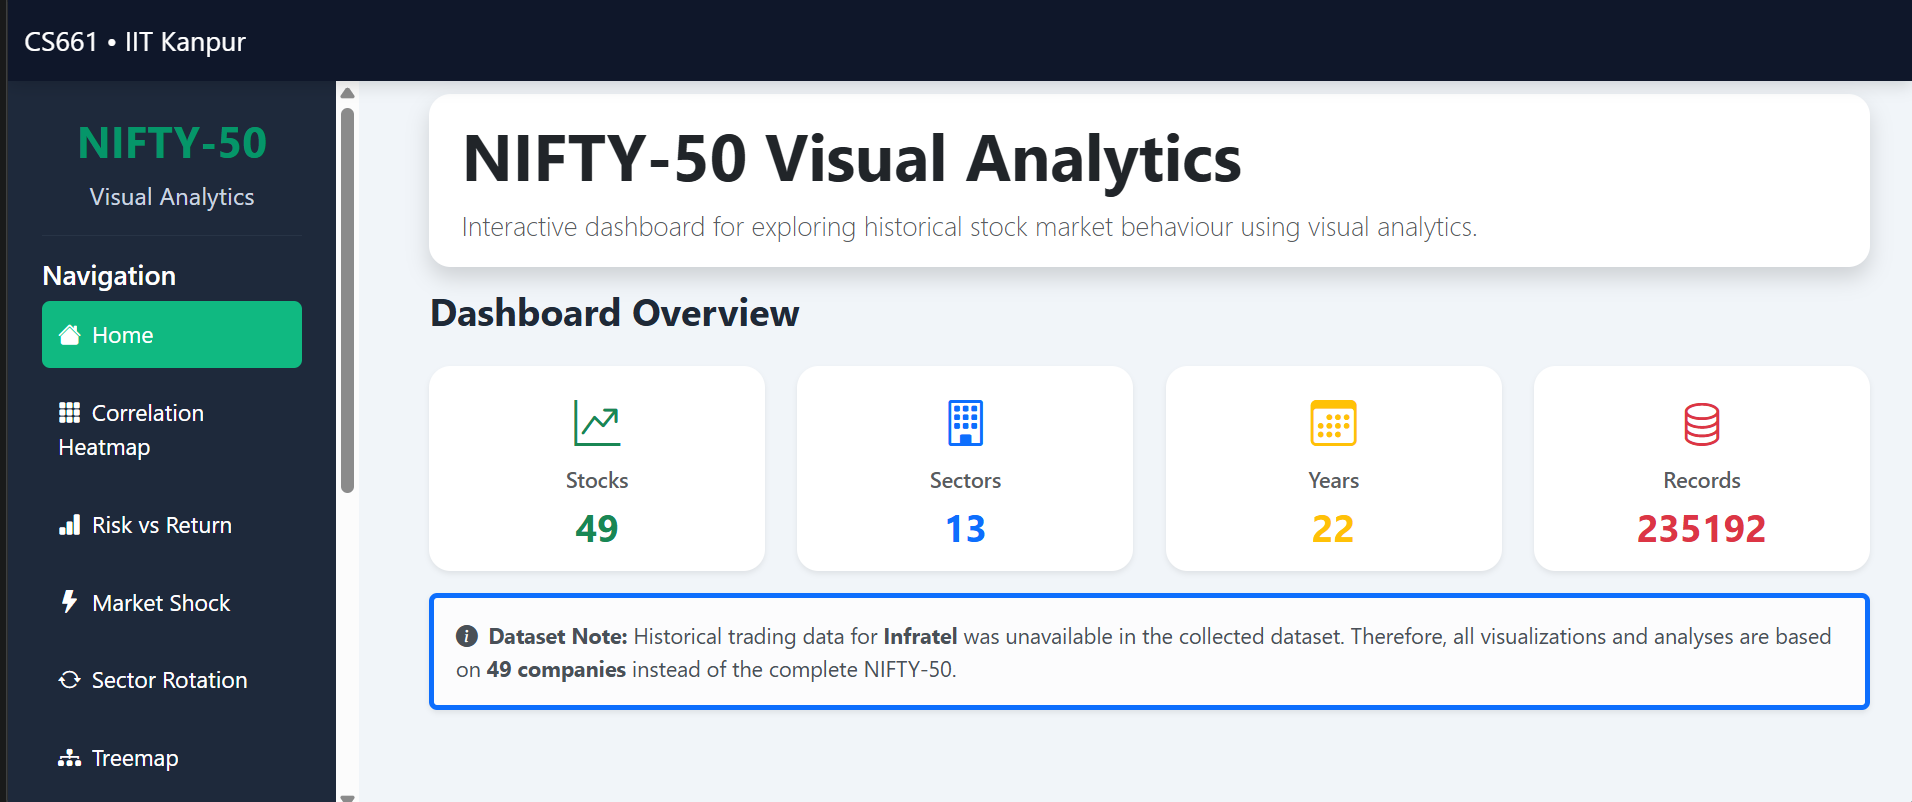
\includegraphics[width=\linewidth]{figures/home.png}
    \caption{Home dashboard -- dataset overview KPI cards and global filters.}
    \label{fig:home}
\end{figure}

\subsection{Information Represented}
\begin{itemize}
    \item Four live KPI cards: total number of stocks, sectors, years of
        coverage, and total records, each recomputed via a DuckDB aggregate
        query as the global filters change.
    \item A hero banner introducing the dashboard.
    \item A data-pipeline explainer (Raw Data \(\rightarrow\) Cleaning
        \(\rightarrow\) Preprocessing \(\rightarrow\) Visual Analytics
        \(\rightarrow\) Insights).
\end{itemize}

\subsection{Observed Trends}
\begin{itemize}
    \item The full dataset spans 49 companies, 13 sectors, and roughly
        21 years of trading history, comprising 235{,}192 records.
    \item Applying sidebar filters (e.g.\ narrowing to a single sector or a
        shorter date range) causes all four KPI cards to update reactively,
        giving an immediate sense of data coverage before drilling into any
        specific analysis.
\end{itemize}

\subsection{Inference and Insights}
\begin{itemize}
    \item Surfacing dataset scale and coverage up front helps users
        calibrate their trust in downstream statistical results (for
        example, correlation or clustering results computed on a
        narrow date range or a sector with very few companies should be
        interpreted with more caution).
    \item Making data limitations (the Infratel exclusion) visible on the
        landing page, rather than burying it in documentation, supports
        transparent and responsible data communication.
\end{itemize}

\subsection{Real-World Implications}
\begin{itemize}
    \item Dashboard designers should surface dataset scope and known gaps
        as a first-class UI element, not an afterthought, especially in
        financial applications where users may make decisions based on the
        data.
    \item Live-updating summary statistics tied to global filters give
        users an implicit sanity check on every subsequent chart they view.
\end{itemize}

\section{Clustered Correlation Matrix Heatmap with Dendrograms}

\subsection{Task Overview}
The goal of this task is to find out which stocks in the NIFTY-50 move
together and which ones move differently, just by looking at their daily
price changes. Normally, if we try to show ``which stock is related to
which other stock'' using a network graph (lines connecting related
stocks), it becomes a big tangled mess when there are 49 stocks --- this is
called a `hairball' because it looks like a ball of hair with no clear
pattern. To avoid this problem, we used a Heatmap combined with a
Dendrogram (a tree diagram) instead. This lets us see the relationship
between every single pair of stocks clearly, and also automatically groups
similar stocks together.

\subsection{Why We Chose Heatmap and Dendrogram Visualization}
We picked the Heatmap + Dendrogram combination for a few simple reasons:

\begin{itemize}
    \item \textbf{No missing connections}: A heatmap is a full grid, so
        every pair of stocks gets a colored cell. Nothing is hidden or
        skipped, unlike a network graph where some lines may overlap or
        get lost.
    \item \textbf{Automatic grouping}: The dendrogram (tree diagram)
        automatically groups stocks that behave similarly, so we do not
        have to manually search for patterns --- the algorithm finds them
        for us.
    \item \textbf{Easy to explore interactively}: The user can select a
        block of stocks directly and instantly see their real
        closing-price history in a separate chart below, without writing
        any code.
\end{itemize}

In short, this visualization was chosen because it is the standard and
most readable way to show relationships among a large number of items
(49 stocks here) without creating visual clutter.

\subsection{How the Data Was Prepared?}
Before we could draw any plot, the raw stock data had to be processed in a
series of steps. Below is what each step does, in simple words:

\noindent\textbf{Step 1 --- Load the Data}

We read the file \texttt{clean\_stock\_data.csv}, which contains the daily
Close price for 49 companies over many years (from year 2000 to 2021).
This file was generated earlier by our data-cleaning scripts
(\texttt{loader.py} and \texttt{preprocessing.py}).

\noindent\textbf{Step 2 --- Compute Daily Returns}

Raw stock prices cannot be compared directly --- for example, a stock
priced at Rs.\ 5000 and a stock priced at Rs.\ 50 are not comparable just
by their price. So instead, we convert each day's price into a percentage
change from the previous day, called the `Daily Return':

\begin{center}
Daily Return = (Today's Close $-$ Yesterday's Close) / Yesterday's Close $\times$ 100
\end{center}

\noindent\textbf{Step 3 --- Create a Pivot Table}

The data is reshaped so that each row is a date, and each column is a
company, with the daily return as the value. This table format is needed
because we want to compare companies (columns) against each other.

\noindent\textbf{Step 4 --- Compute the Correlation Matrix}

For every pair of stocks, we calculate how similarly their daily returns
moved, using a statistic called Correlation. The value ranges from $-1$ to
$+1$: a value close to $+1$ means the two stocks moved together most days,
a value close to $-1$ means they moved in opposite directions, and a value
close to 0 means there is no clear relationship.

\noindent\textbf{Step 5 --- Hierarchical (Agglomerative) Clustering}

Using the correlation values, we group similar stocks together using a
technique called Agglomerative Clustering (from the scikit-learn library).
Since clustering needs a `distance' instead of a `correlation' (they are
opposite ideas), we convert correlation into distance using the formula:
\textbf{Distance = 1 $-$ Correlation}. A high correlation therefore means a
very small distance, so those two stocks are considered `close' to each
other. We also use the SciPy library to build the tree structure required
to actually draw the dendrogram diagram.

\noindent\textbf{Step 6 --- Reorder the Heatmap}

Finally, the original correlation matrix is reordered --- both its rows
and its columns --- to match the order that stocks appear in the
dendrogram tree. This is the step that makes similar stocks appear next to
each other in the heatmap, turning a random-looking grid into one with
clear, visible blocks.

\subsection{The Visualizations --- What Each Plot Shows?}

\noindent\textbf{Figure 1: Hierarchical Clustering Dendrogram}

This tree diagram shows how stocks get grouped together, step by step.
Every stock starts as its own branch at the bottom. Two branches join
together at a certain height, and that height tells us how different
those two stocks (or groups of stocks) are:

\begin{itemize}
    \item \textbf{Low join} (near the bottom) means the two stocks are
        highly correlated --- they moved together very closely.
    \item \textbf{High join} (near the top) means the two stocks or
        groups are only loosely related, and got joined mainly because
        the algorithm eventually merges everything into one big tree.
    \item The colors (red, purple, orange, green, etc.) do not carry any
        special meaning by themselves --- they are only used to visually
        separate distinct clusters so the eye can tell them apart. The
        important information is the height of the join, not the color.
\end{itemize}

\begin{figure}[h!]
    \centering
    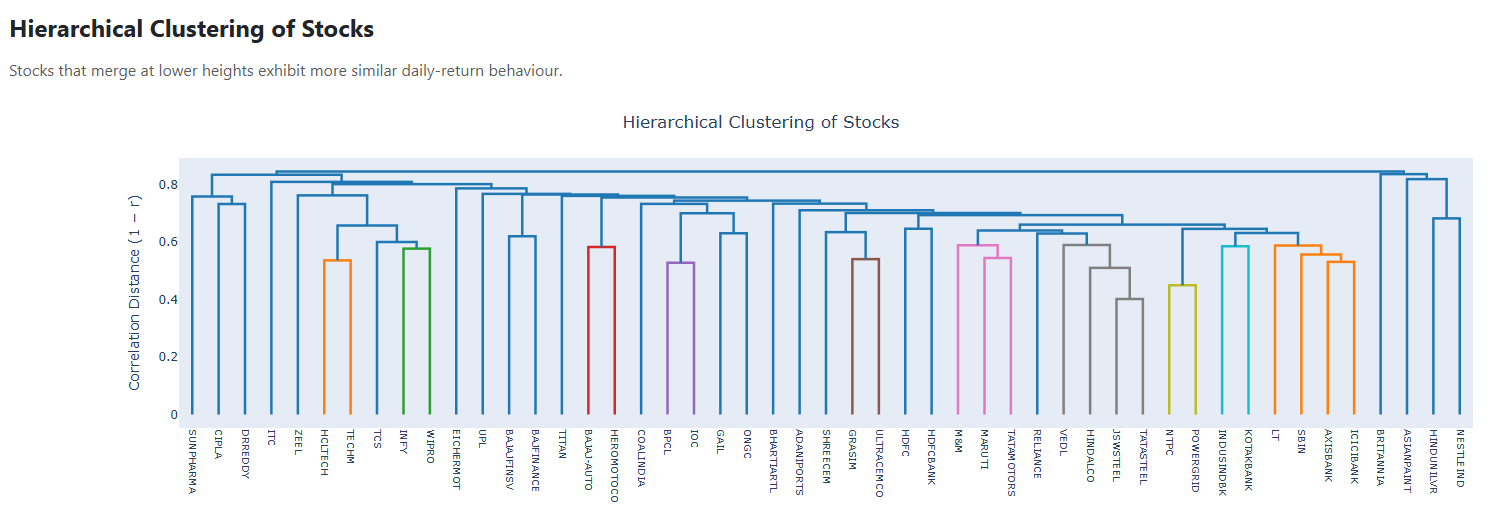
\includegraphics[width=\linewidth]{figures/correlation_dendrogram.png}
    \caption{Dendrogram showing how the 49 NIFTY-50 stocks group together based on similarity of daily returns.}
    \label{fig:correlation_dendrogram}
\end{figure}

\noindent\textbf{Figure 2: Clustered Correlation Heatmap}

This is a 49 $\times$ 49 grid, where both the rows and the columns are
stock names, arranged in the same order as the dendrogram above. Each
small square (cell) is colored based on the correlation value between the
row-stock and column stock. By clicking on each cell we get correlation
value between two companies.

\begin{itemize}
    \item \textbf{Dark Red} = strong positive correlation (moved
        together).
    \item \textbf{White} = almost no relationship (correlation close to
        0).
    \item \textbf{Blue} = negative correlation (moved in opposite
        directions).
\end{itemize}

The diagonal line running from top-left to bottom-right is always the
darkest red, because every stock is perfectly correlated with itself
(correlation = 1).

\begin{figure}[h!]
    \centering
    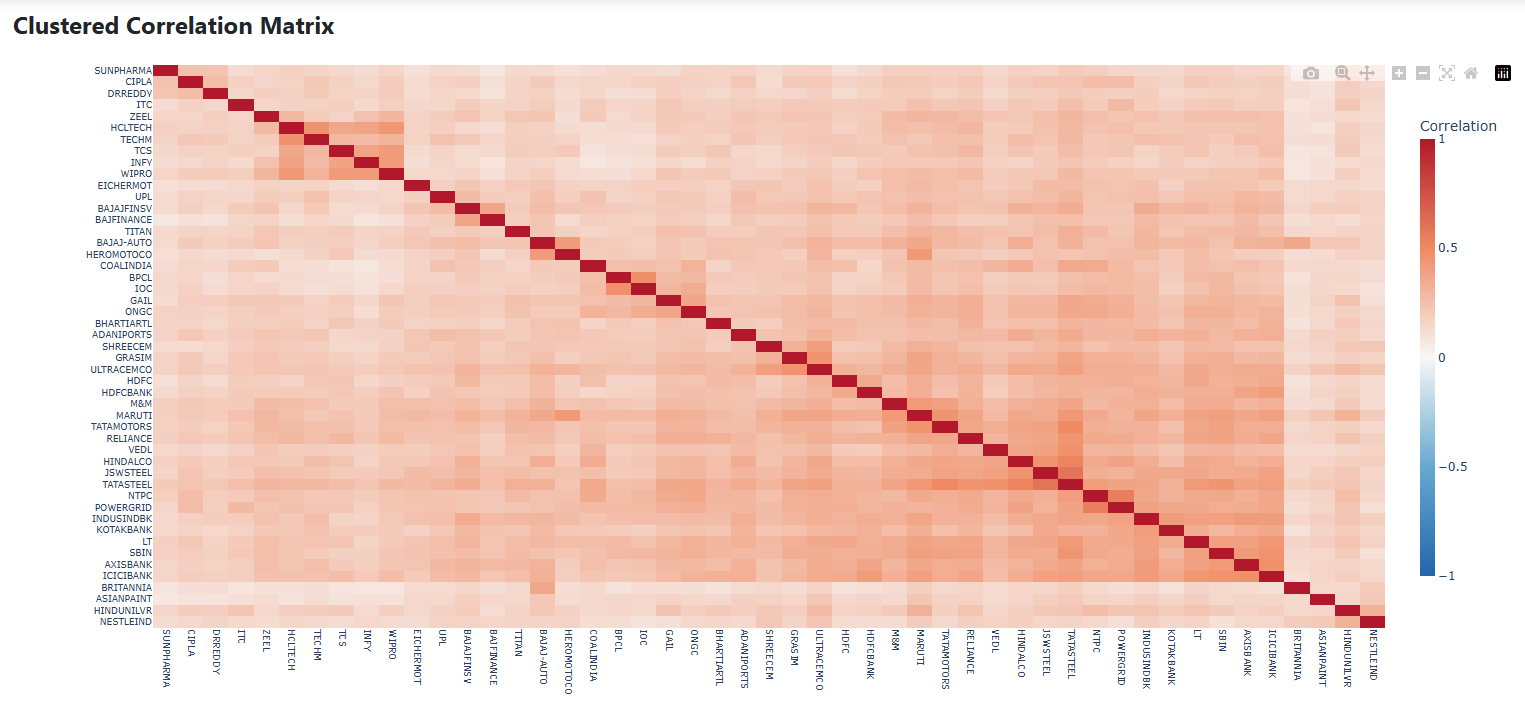
\includegraphics[width=\linewidth]{figures/correlation_heatmap.png}
    \caption{Clustered correlation heatmap. Notice the small dark red blocks near the diagonal --- these are groups of stocks that move together, matching the clusters seen in the dendrogram above.}
    \label{fig:correlation_heatmap}
\end{figure}

\noindent\textbf{Figure 3: Closing Price Comparison}

This line chart sits below the heatmap and shows the actual closing price
history of whichever stocks are currently selected. It is directly linked
to the heatmap above: if the user drags the mouse to select a block of
cells on the heatmap (this is called `brushing'), the stock names under
that selection automatically appear in this chart, so the user can
immediately verify with real price data whether the correlation actually
makes sense.

\begin{figure}[h!]
    \centering
    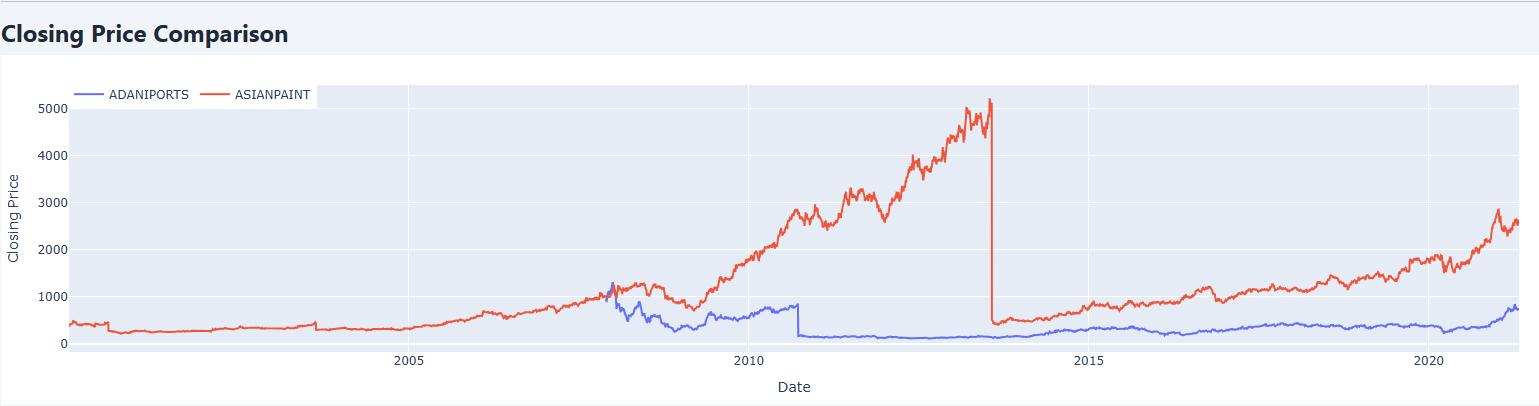
\includegraphics[width=\linewidth]{figures/correlation_price_comparison.png}
    \caption{Closing price comparison for ADANIPORTS and ASIANPAINT, shown after selecting them from the heatmap/dropdown.}
    \label{fig:correlation_price_comparison}
\end{figure}

\subsection{Interactive Features}
\begin{itemize}
    \item \textbf{Number of Clusters Slider:} Lets the user choose how
        many groups (from 2 to 10) the clustering algorithm should split
        the stocks into. Changing this value re-runs the clustering and
        updates the colors in the dendrogram.
    \item \textbf{Company Dropdown:} Allows users to search and select a
        specific company to visualize how its stock's closing price
        changes over time.
    \item \textbf{Brushing on the Heatmap:} The user can click on
        rectangle over a block of cells in the heatmap and easily find the
        correlation between the companies.
\end{itemize}

These features together make the dashboard exploratory: a user does not
need to already know which stocks are related --- they can simply look at
the picture, click on an interesting-looking block, and instantly see if
the underlying price data supports that pattern.

\subsection{What We Observed (Trends)}
\begin{itemize}
    \item \textbf{Pharma stocks cluster together}: SUNPHARMA, CIPLA, and
        DR.\ REDDY forms a tight, clearly visible group at the very start
        of the heatmap and dendrogram. This makes sense because
        pharmaceutical companies tend to be affected by similar factors,
        such as drug approvals or export policies.
    \item \textbf{IT stocks cluster together:} HCLTECH, TECHM, TCS, INFY,
        and WIPRO form another visible group. These companies share the
        same industry drivers, such as the US dollar exchange rate and
        global technology spending.
    \item \textbf{FMCG stocks cluster together}: ASIANPAINT, HINDUNILVR,
        and NESTLEIND form their own small cluster near the end of the
        heatmap, since consumer-goods companies often react similarly to
        changes in consumer spending.
    \item \textbf{Most correlations are mild, not extreme:} Looking at the
        heatmap, most cells (outside the diagonal) are light orange,
        meaning correlation values are mostly in the 0.1 to 0.3 range
        rather than very high or very low. This is expected --- these are
        all large, well-established companies that are all somewhat
        influenced by the overall Indian stock market, but each also has
        its own company-specific ups and downs.
    \item \textbf{Very little negative correlation:} Almost no cell in
        the heatmap is blue. This means it is rare for two NIFTY-50 stocks
        to move in completely opposite directions on the same day ---
        again expected, since broad market movements tend to push most
        large stocks in the same general direction.
\end{itemize}

\subsection{Why This Matters (Real-World Use)}
\begin{itemize}
    \item \textbf{Portfolio diversification:} An investor can use this
        visualization to avoid picking stocks that are all from the same
        cluster (for example, all pharma stocks). Choosing stocks from
        different clusters spreads out risk, because those stocks are
        less likely to fall at the same time.
    \item \textbf{Finding hidden relationships:} Some stocks may be
        correlated for reasons that go beyond their official `sector'
        label (for example, two companies that both depend heavily on
        oil prices, even if they are in different industries). This
        visualization can reveal such hidden relationships that a simple
        sector-based grouping would miss.
    \item \textbf{Faster exploration of large data:} With 49 stocks,
        there are 49 $\times$ 49 = 2,401 correlation values to look at.
        Reading these as raw numbers in a table would be extremely slow
        and error-prone. A single glance at the heatmap and dendrogram
        gives the same information almost instantly.
\end{itemize}

\subsection{Conclusion}
This task successfully builds an interactive dashboard page that turns a
large, hard-to-read correlation table into an easy-to-understand visual: a
heatmap for seeing every pairwise relationship at a glance, and a
dendrogram for automatically grouping similar stocks. The two are linked
together with an interactive time-series chart, allowing a user to go from
a broad visual pattern all the way down to actual daily closing prices in
just one click. The backend logic (\texttt{utils/analytics/correlation.py})
and the dashboard page (\texttt{pages/correlation.py}) were built using
pandas, scikit-learn, SciPy, and Plotly, exactly as required for this task.

\section{Risk--Return Analysis}

\subsection{Task Overview}
The relationship between risk and return is one of the fundamental
concepts in financial analysis. While investors generally seek higher
returns, achieving those returns often requires accepting greater
investment risk. Therefore, evaluating return without considering risk
may lead to misleading investment decisions.

This dashboard analyzes the historical performance of NIFTY-50 companies
by computing annualized return and annualized volatility for each stock.
These two metrics are visualized using an interactive scatter plot, where
every point represents one company. Companies with similar risk-return
characteristics are automatically grouped using the K-Means clustering
algorithm.

To complement the scatter plot, a linked cumulative return chart allows
users to compare the historical performance of any selected company with
the NIFTY-50 benchmark. Together, these visualizations provide both a
high-level overview of market risk profiles and a detailed view of
long-term stock performance.

\subsection{Why We Chose Scatter Plot and Cumulative Return Chart Visualizations}
Financial data naturally involves multiple variables that should be
interpreted simultaneously. A scatter plot provides an effective way to
visualize the relationship between annual return and annual volatility
for every company in a single figure. Unlike tables, it immediately
reveals patterns, clusters, and outliers.

To complement the scatter plot, a cumulative return chart was selected
because it shows how an investment grows over time. Linking both
visualizations allows users to move from a high-level market overview to
detailed historical performance with a single click.

\subsection{How the Data Was Prepared}

\noindent\textbf{Step 1 --- Load the Data}

Daily closing prices of all NIFTY-50 companies are loaded from the
cleaned dataset.

\noindent\textbf{Step 2 --- Compute Daily Returns}

For every company, daily percentage returns are calculated using

\begin{center}
Daily Return $= \dfrac{P_t - P_{t-1}}{P_{t-1}}$
\end{center}

where $P_t$ represents the closing price on the current trading day.

\noindent\textbf{Step 3 --- Calculate Annualized Return}

The average daily return is multiplied by 252 (average trading days in
one year):

\begin{center}
Annual Return $= \text{Mean}(\text{Daily Return}) \times 252$
\end{center}

\noindent\textbf{Step 4 --- Calculate Annualized Volatility}

Risk is measured using the standard deviation of daily returns.

\begin{center}
Annual Volatility $= \text{Std}(\text{Daily Return}) \times \sqrt{252}$
\end{center}

Higher volatility indicates larger price fluctuations and therefore
higher investment risk.

\noindent\textbf{Step 5 --- Feature Scaling}

Since annual return and annual volatility have different numerical
ranges, both features are standardized using the StandardScaler before
clustering.

\noindent\textbf{Step 6 --- K-Means Clustering}

The standardized data is grouped into four clusters using the K-Means
algorithm. Each cluster represents companies having similar combinations
of return and risk.

\noindent\textbf{Step 7 --- Dynamic Risk Profile Assignment}

Since K-Means assigns arbitrary cluster IDs, each cluster is analyzed
according to its average annual return and annual volatility before
assigning descriptive labels such as:

\begin{itemize}
    \item High Risk, High Return
    \item High Risk, Low Return
    \item Moderate Risk, Steady Return
    \item Defensive / Low Volatility
\end{itemize}

This ensures that the interpretation remains correct even after applying
filters or changing the selected date range.

\subsection{The Visualizations}

\subsubsection{Figure 1: Risk vs Return Scatter Plot}

Each point represents one company.

\begin{itemize}
    \item X-axis represents Annual Volatility (Risk).
    \item Y-axis represents Annual Return.
    \item Different colors represent different K-Means clusters.
    \item Dotted horizontal and vertical lines represent average market
        return and average market risk.
    \item Hovering over a point displays company name, sector, annual
        return, annual volatility, and assigned risk profile.
\end{itemize}

\begin{figure}[h!]
    \centering
    \includegraphics[width=\linewidth]{figures/risk_return_scatter.png}
    \caption{Risk vs Return Scatter Plot showing clustered NIFTY-50 companies based on annualized return and annualized volatility.}
    \label{fig:risk_return_scatter}
\end{figure}

\subsubsection{Figure 2: Company vs NIFTY-50 Cumulative Return}

When a company is selected from the scatter plot, its cumulative return
is displayed alongside the NIFTY-50 average.

The chart illustrates how the value of an investment of 100 grows over
time for both the selected company and the benchmark index. This enables
users to compare long-term performance against the market.

\begin{figure}[h!]
    \centering
    \includegraphics[width=\linewidth]{figures/risk_return_cumulative.png}
    \caption{Comparison of cumulative return between the selected company and the NIFTY-50 benchmark.}
    \label{fig:risk_return_cumulative}
\end{figure}

\subsection{Interactive Features}
\begin{itemize}
    \item \textbf{Scatter Plot Selection:} Clicking any company highlights
        it while fading the remaining companies.
    \item \textbf{Linked Visualization:} Selecting a company automatically
        updates the cumulative return chart.
    \item \textbf{Hover Information:} Users can inspect company name,
        sector, annual return, annual volatility, and assigned risk
        profile.
    \item \textbf{Date Filters:} Risk and return statistics are
        recalculated dynamically for the selected period.
    \item \textbf{Sector and Company Filters:} Users can analyze either
        the complete market or specific sectors and companies.
    \item \textbf{Reset View Button:} Restores the original visualization
        and clears the selected company.
    \item \textbf{Zoom and Pan:} Users can zoom into the scatter plot and
        reset the axes using Plotly's interactive toolbar.
\end{itemize}

\noindent\textbf{Linked Interaction Example}

Figure~\ref{fig:risk_return_linked} demonstrates the interactive linking
implemented in the dashboard. Selecting a company in the Risk--Return
scatter plot highlights the chosen company while reducing the opacity of
the remaining points. At the same time, the cumulative return chart
updates to compare the selected company's historical performance against
the NIFTY-50 benchmark.

\begin{figure}[h!]
    \centering
    \begin{minipage}{0.48\linewidth}
        \centering
        \includegraphics[width=\linewidth]{figures/risk_return_linked_scatter.png}
        \caption*{(a) Scatter plot after selecting a company}
    \end{minipage}
    \hfill
    \begin{minipage}{0.48\linewidth}
        \centering
        \includegraphics[width=\linewidth]{figures/risk_return_linked_cumulative.png}
        \caption*{(b) Corresponding cumulative return comparison}
    \end{minipage}
    \caption{Linked interaction between the Risk--Return scatter plot and the cumulative return chart. Selecting a company in the scatter plot automatically updates the cumulative return visualization while highlighting the selected company.}
    \label{fig:risk_return_linked}
\end{figure}

Some important observations from the visualization include:

\begin{itemize}
    \item Companies with higher annual returns generally exhibit higher
        annual volatility, illustrating the classical risk-return
        trade-off.
    \item Defensive companies appear in the lower-left region of the
        scatter plot, indicating relatively lower risk and stable returns.
    \item Some companies generate high returns but also experience
        considerably larger price fluctuations.
    \item K-Means clustering clearly separates companies into distinct
        investment profiles, making comparison much easier than examining
        numerical statistics alone.
    \item Comparing cumulative returns with the NIFTY-50 benchmark
        quickly reveals which companies consistently outperform the
        overall market.
\end{itemize}

\subsection{Why This Matters (Real-World Use)}
\begin{itemize}
    \item Investors can compare expected return against investment risk
        before selecting stocks.
    \item Portfolio managers can diversify investments by selecting
        companies from different risk clusters.
    \item Benchmark comparison helps identify companies that consistently
        outperform the overall market.
    \item Financial analysts can quickly evaluate whether a company's
        return justifies the level of investment risk it carries.
\end{itemize}

\subsection{Conclusion}
This task successfully develops an interactive dashboard for analyzing
the relationship between risk and return among NIFTY-50 companies. By
combining annualized return, annualized volatility, K-Means clustering,
and linked cumulative return visualization, the dashboard enables users
to explore investment characteristics intuitively. Interactive filtering,
company selection, benchmark comparison, and linked visualizations
transform complex financial statistics into an easy-to-understand visual
analytics tool for portfolio analysis and investment decision-making.

\section{Market Shock \& Systemic Anomaly Detection}

\subsection{Task Overview}
Financial markets are periodically subjected to extreme volatility, often
driven by macroeconomic events, geopolitical crises, or sudden shifts in
investor sentiment. While normal market analysis looks at long-term growth,
risk management requires understanding how a portfolio behaves during these
sudden ``shocks.''

The goal of this task is to automatically detect extreme market events
(both crashes and rallies) across historical data and measure their
systemic severity. Furthermore, it allows users to drill down into any
specific day of crisis to observe the cross-sectional dispersion of the
market. This reveals whether a crash was a market-wide panic
(\textit{systemic}) or isolated to a few specific industries
(\textit{idiosyncratic}).

\subsection{Why We Chose Diverging Timeline and Beeswarm Visualizations}
To effectively analyze market shocks, we needed to provide both a macro
(long-term historical) and micro (single-day cross-sectional) perspective.
We chose specific visual layouts to avoid the pitfalls of standard
charting methods:

\begin{itemize}[label=-]
    \item \textbf{Diverging Timeline Heatmap (Macro View):} Standard line
        charts of stock prices mask underlying volatility, making it hard
        to spot a 5\% drop if the overall market is trending upward. We
        chose a diverging bar chart to represent aggregate market severity.
        By plotting market crashes as negative (red bars pointing downward)
        and rallies as positive (green bars pointing upward), the
        visualization taps into intuitive financial psychology. Analysts
        can scan 15+ years of data and instantly spot periods of severe
        market distress.
    \item \textbf{Beeswarm / Strip Plot (Micro View):} When analyzing a
        single day's shock, we need to see how every individual company
        reacted. Box plots hide outliers (which are the most important
        part of a crisis), and standard scatter plots result in heavily
        overlapping dots. A Beeswarm plot spreads the data points out
        horizontally within their respective sectors, ensuring every
        single company remains visible and can be hovered over for exact
        details.
\end{itemize}

\subsection{How the Data Was Prepared?}
Before we could draw any plot, the raw stock data had to be mathematically
standardized. To ensure the application remains highly responsive even
with hundreds of thousands of rows of data, the data preparation is pushed
down to a highly optimized \textbf{DuckDB} SQL engine rather than relying
on Pandas, which would quickly exhaust the server's RAM.

\begin{itemize}[label=]

\item \textbf{Step 1: Load the Data}\\
Daily closing prices and sector classifications for all NIFTY-50 companies
are queried directly from the persistent \texttt{clean\_stock\_data} table.

\item \textbf{Step 2: Calculate Rolling Statistics}\\
Raw price drops cannot be compared directly across different timelines. A
volatile day in a quiet year like 2014 looks very different from a normal
day during the 2008 financial crisis. To account for changing market
regimes, we calculate a rolling moving average ($\mu$) and rolling
standard deviation ($\sigma$) for every stock over a user-defined window
(defaulting to 20 days) using SQL Window Functions.

\item\textbf{Step 3: Compute Z-Scores}
Instead of looking at raw price changes, we standardize the daily closing
price into a Z-Score. This metric measures how many standard deviations a
stock's price is from its recent moving average:
\begin{equation}
Z = \frac{\text{Close} - \mu}{\sigma}
\end{equation}
A Z-Score of -3.0 indicates a severe, statistically significant drop (a
crash), while +3.0 indicates a severe rally. This puts all
stocks---regardless of their actual share price---on a level playing
field.

\item \textbf{Step 4: Threshold Filtering \& Aggregation}\\
Based on the user's selected Z-Score threshold, the DuckDB backend uses
\texttt{CASE WHEN} statements to count how many companies experienced an
anomaly on a given day. The final ``Severity Score'' for the market is
calculated by multiplying the number of anomalous companies by their
average Z-Score on that day.

\item \textbf{Step 5: Stateless Query Execution}\\
Using Common Table Expressions (CTEs), the entire mathematical pipeline is
executed on-the-fly. When a user interacts with the dashboard, Dash sends
a lightweight SQL string to DuckDB, which instantly aggregates the exact
X/Y coordinates needed for the charts in milliseconds.
\end{itemize}

\subsection{The Visualizations}

\textbf{Figure 1: Systemic Market Volatility (Diverging Timeline)}\\
This bar chart shows the historical aggregate health of the NIFTY-50
market.
\begin{itemize}[label=-]
    \item \textbf{X-axis:} Date (Trading days over the historical
        dataset).
    \item \textbf{Y-axis:} Severity Score (Number of crashing/rallying
        stocks multiplied by their average volatility).
    \item \textbf{Red Bars (Negative):} Represent Market Crashes. The
        deeper the bar goes, the more severe and widespread the panic on
        that day.
    \item \textbf{Green Bars (Positive):} Represent Market Rallies.
\end{itemize}

\begin{figure}[H]
    \centering
    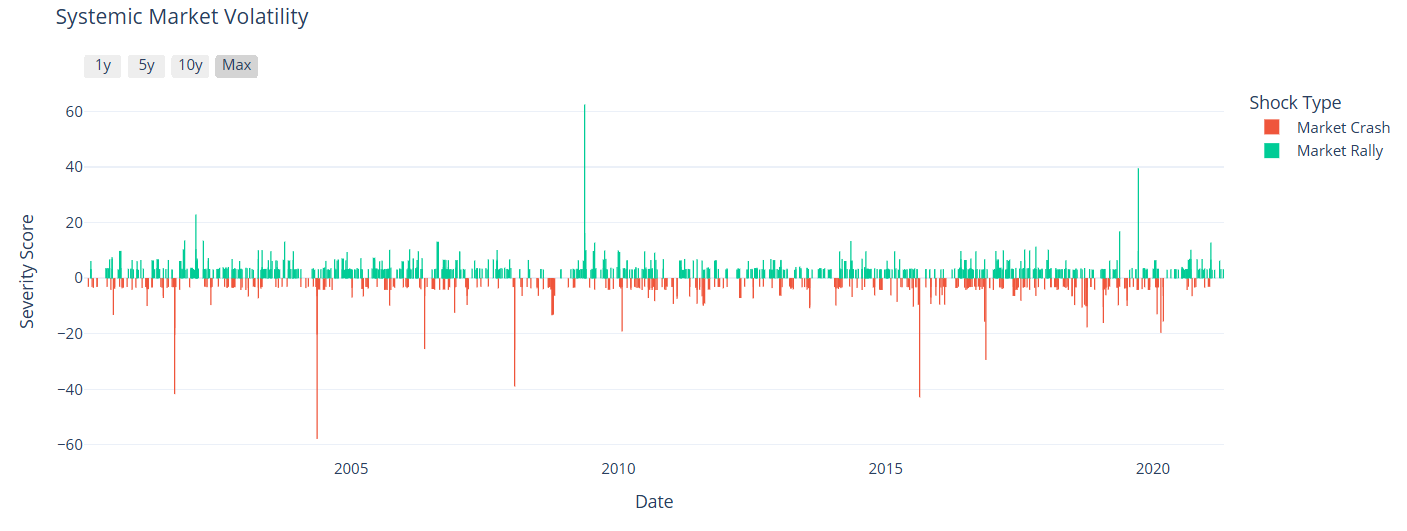
\includegraphics[width=1\linewidth]{figures/market_shock_timeline.png}
    \caption{Systemic Market Volatility (Diverging Timeline) aggregating the severity of daily market shocks across NIFTY-50 companies over 15 years. Market crashes are represented by negative red bars, while rallies are represented by positive green bars. Data is filtered using a Z-Score anomaly threshold of $\pm 3.0$ and a rolling statistical window of 20 days.}
    \label{fig:market_shock_timeline}
\end{figure}

\textbf{Figure 2: Sector Dispersion (Beeswarm Plot)}\\
This chart sits below the timeline and shows the exact anatomy of the
market for one specific chosen date.
\begin{itemize}[label=-]
    \item \textbf{X-axis:} Market Sectors (e.g., Financial Services, IT,
        Pharma).
    \item \textbf{Y-axis:} Volatility (Z-Score) for the selected date.
    \item \textbf{Data Points:} Each dot represents a single company,
        colored by its sector.
    \item \textbf{Reference Lines:} Dynamic dashed red lines show the
        current anomaly threshold (e.g., $+3.0\sigma$ and $-3.0\sigma$),
        making it instantly clear which specific companies breached the
        threshold.
\end{itemize}

\begin{figure}[H]
    \centering
    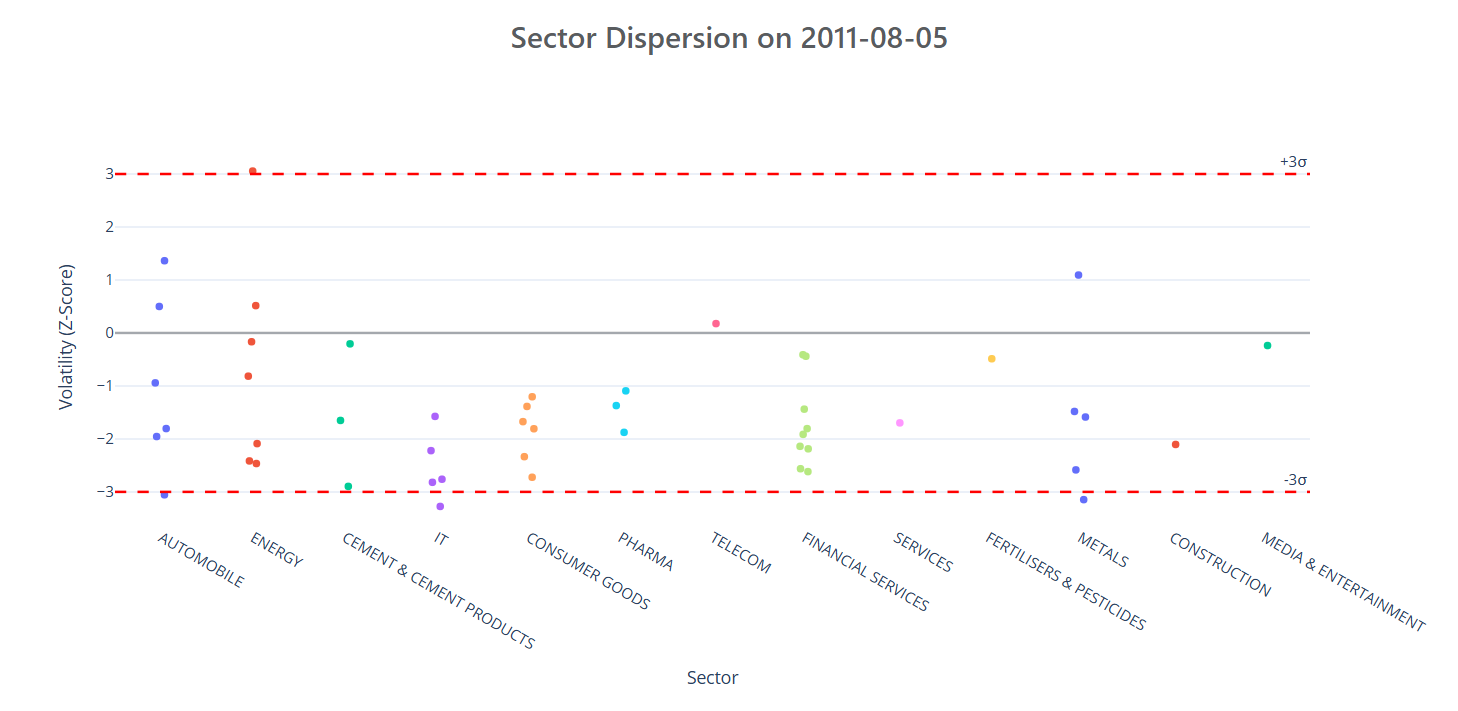
\includegraphics[width=1\linewidth]{figures/market_shock_beeswarm.png}
    \caption{Sector Dispersion (Beeswarm Plot) detailing the cross-sectional volatility of individual NIFTY-50 companies on August 5, 2011. Each data point represents a single company, colored by its sector. The dynamic dashed red lines indicate the active anomaly threshold ($\pm 3.0\sigma$) over a 20-day rolling window, highlighting the widespread systemic nature of the shock on this specific date.}
    \label{fig:market_shock_beeswarm}
\end{figure}

\subsection{Interactive Features}
\begin{itemize}[label=-]
    \item \textbf{Anomaly Threshold Slider:} Allows the user to define
        what constitutes a ``shock.'' Lowering the threshold (e.g., 2.0)
        reveals minor market corrections, while raising it (e.g., 4.0)
        filters out the noise to isolate only true historical black-swan
        events.
    \item \textbf{Rolling Window Slider:} Adjusts the ``memory'' of the
        baseline statistics (from 10 to 60 days). A 10-day window
        highlights rapid short-term shocks, while a 60-day window
        highlights longer-term regime shifts.
    \item \textbf{Interactive Calendar Syncing:} A native Date Picker
        widget allows users to manually look up specific historical
        dates. To prevent errors, a background query calculates all
        weekends and non-trading holidays and explicitly disables (grays
        out) those invalid dates in the calendar.
    \item \textbf{Cross-Filtering (Brushing):} The timeline and the
        beeswarm plot are perfectly linked. Clicking any red or green
        spike directly on the timeline heatmap instantly updates the
        calendar widget and renders that specific day's dispersion on the
        Beeswarm plot below.
    \item \textbf{Native Zoom State Preservation:} Users can click and
        drag to zoom into specific historical periods (e.g., just the
        2020 pandemic) on the timeline. Adjusting the sliders recalculates
        the math without resetting the user's zoom level, allowing for
        seamless deep-dive exploration.
\end{itemize}

\subsection{What We Observed (Trends)}
\begin{itemize}[label=-]
    \item \textbf{The 2008 \& 2020 Crises:} The diverging timeline clearly
        highlights massive, systemic downward spikes during the 2008
        Global Financial Crisis and the March 2020 COVID-19 sell-off.
        Clicking on these dates reveals a Beeswarm plot where almost every
        sector plunged simultaneously across the $-3.0\sigma$ line,
        proving they were true \textit{systemic} macroeconomic shocks.
    \item \textbf{Sector Rotations (Idiosyncratic Shocks):} On certain
        dates outside of global crises, the Beeswarm plot reveals isolated
        shocks. For example, selecting a specific day might show the IT
        sector with extreme negative Z-scores due to global tech
        sell-offs, while Defensive sectors like FMCG remain perfectly
        clustered near the $0\sigma$ baseline.
\end{itemize}

\subsection{Why This Matters (Real-World Use)}
\begin{itemize}[label=-]
    \item \textbf{Stress Testing:} Portfolio managers can use this tool to
        look up specific historical crisis days and see exactly how their
        current holdings would have reacted to similar market distress.
    \item \textbf{Contagion Analysis:} Analysts can determine if a shock
        in one specific sector (e.g., a banking collapse) bled over into
        other sectors, or if it remained successfully isolated.
    \item \textbf{Volatility Targeting:} By adjusting the rolling window
        and threshold sliders, quantitative analysts can refine the
        mathematical parameters they use for algorithmic trading safety
        mechanisms and risk models.
\end{itemize}

\subsection{Conclusion}
This task successfully transforms highly dense, complex volatility data
into an intuitive visual engine. By utilizing a stateless DuckDB backend,
the dashboard avoids memory bottlenecks and can process rolling
calculations on-the-fly. The combination of a macro-level diverging
timeline and a micro-level cross-sectional beeswarm plot allows users to
seamlessly navigate from a 15-year historical market view all the way down
to the behavior of a single stock on a specific day of crisis.

\section{Sector Rotation \& Capital Flow Dynamics}

\subsection{Task Overview}
This task studies how capital rotates between sectors relative to the
broader NIFTY-50 market, using a Relative Rotation Graph (RRG). Rather than
tracking each sector's absolute performance in isolation, the goal is to
answer: \textit{is this sector currently gaining strength relative to the
market, and is that strength accelerating or fading?} The backend computes
normalized sector indices, a market benchmark, Relative Strength (RS),
RS-Ratio, and RS-Momentum, and classifies every sector-week into one of
four quadrants --- \textbf{Leading, Weakening, Lagging, Improving}.
Quadrant assignment is recalculated at every time step, not fixed per
sector. A sector's position moves across the plot as its RS-Ratio and
RS-Momentum evolve, and the frontend animates this movement, which is the
entire purpose of an RRG.

\subsection{Why We Chose the Relative Rotation Graph}
A multi line chart of 13 sector indices over 20 years becomes unreadable
quickly, since all sectors tend to trend upward together during bull
markets, hiding \textit{relative} performance. The RRG solves this by
re-centering everything around the market average (RS-Ratio = 100,
RS-Momentum = 0), so a sector's position and direction of travel directly
answers ``is this sector in favor right now, and is that changing?'' We
chose this over a plain performance table because:

\begin{itemize}
    \item \textbf{Two dimensions in one glance}: trend strength (RS-Ratio)
        and momentum (RS-Momentum) are shown together.
    \item \textbf{Rotational storytelling}: sectors visibly travel Lagging
        \(\rightarrow\) Improving \(\rightarrow\) Leading \(\rightarrow\)
        Weakening \(\rightarrow\) Lagging in cycles, a commonly used
        framework in quantitative finance for analyzing sector rotation.
    \item \textbf{Directly comparable to market}: both axes are rebased to
        the market benchmark, so all sectors sit on a common, interpretable
        scale.
\end{itemize}

\subsection{How the Data Was Prepared}
The cleaned dataset (\texttt{Company, Sector, Date, Close}) is validated on
load. Each company's closing price is rebased to 100 at its first available
date, and averaged within its sector to form an equal-weighted normalized
Sector Index --- reflecting the average performance of companies in the
sector rather than being dominated by high nominal share prices. A Market
Index is built the same way across all companies, so no external benchmark
file is needed. Both series are rebased to 100 again at their first common
date before computing:

\begin{align*}
    \textbf{RS} &= (\text{SectorIndex} / \text{MarketIndex}) \times 100 \\
    \textbf{RS-Ratio} &= (\text{RS} / \text{RollingMean}(\text{RS}, 14)) \times 100 \\
    \textbf{RS-Momentum} &= ((\text{RS-Ratio}_t / \text{RS-Ratio}_{(t-10)}) - 1) \times 100
\end{align*}

Rebasing removes the influence of absolute stock price levels, letting
sectors with very different price ranges be compared fairly. The 14-day and
10-day rolling windows are computed on daily data before weekly
resampling, preserving the intended time horizon. Computing them after
resampling would incorrectly stretch the signal over a much longer period.
The first \texttt{window} rows of each sector are left unclassified
(quadrant = \texttt{None}) until enough history exists for a stable rolling
calculation. All stages are vectorized Pandas operations
(\texttt{groupby().transform()}, \texttt{rolling}, \texttt{shift}), so the
pipeline scales linearly (\(O(n)\)) with the number of rows, which keeps it
responsive even across 20+ years of daily data.

\subsection{The Visualizations}

\begin{figure}[h!]
    \centering
    \includegraphics[width=\linewidth]{figures/sector_rotation.png}
    \caption{Animated Relative Rotation Graph. The RRG scatter plot showing all 13 NIFTY sectors positioned by RS-Ratio (x-axis) and RS-Momentum (y-axis) at the animation frame ending 2021-04-26.}
    \label{fig:sector_rotation}
\end{figure}

A 2D scatter plot with RS-Ratio on the x-axis and RS-Momentum on the y-axis,
split into four quadrants by dashed lines at x=100 and y=0. Each of the 13
sectors is a colored dot. A play/pause control and date slider let the user
scrub through weekly snapshots or auto-animate the rotation, with a Time
Horizon filter (1M/3M/6M/1Y/All) controlling how much history is shown.
Hovering any dot reveals exact values. E.g., at the frame dated 2021-04-26,
CEMENT \& CEMENT PRODUCTS shows RS-Ratio = 95.95, RS-Momentum = $-6.03$,
while FINANCIAL SERVICES shows RS-Ratio = 109.18, RS-Momentum = 13.73.

\begin{figure}[h!]
    \centering
    \includegraphics[width=\linewidth]{figures/sector_rotation_deep_dive.png}
    \caption{Sector Deep Dive. The Sector Deep Dive panel showing a selected sector's full 2000--2021 RS-Ratio and RS-Momentum decomposition.}
    \label{fig:sector_rotation_deep_dive}
\end{figure}

Clicking any sector dot loads a linked panel with two stacked time-series
charts: RS-Ratio and RS-Momentum across the full 2000--2021 history,
letting the user check whether a sector's current position is consistent
with its long-run behavior, rather than relying solely on the instantaneous
RRG position.

\subsection{Interactive Features}
\begin{itemize}
    \item \textbf{Time Horizon Filter}: 1M/3M/6M/1Y/All radio buttons to
        zoom the animation window.
    \item \textbf{Play/Pause Animation \& Date Slider}: auto-play the
        rotation or scrub directly to any week.
    \item \textbf{Click-to-Drill-Down}: loads a sector's full historical
        decomposition into the Sector Deep Dive panel.
    \item \textbf{Hover Tooltips}: exact Sector, PeriodStr, RS\_Ratio, and
        RS\_Momentum values per frame.
    \item \textbf{Sidebar Filters}: Start Date, End Date, Sector, and
        Company dropdowns for narrowing the view.
\end{itemize}

\subsection{What We Observed (Trends)}
Quadrant assignments are dynamic. A sector's position is a snapshot, not a
permanent label, and the animation lets users watch it change over time. At
the frame ending 2021-04-26, \textbf{FINANCIAL SERVICES} lay in the Leading
quadrant (RS-Ratio 109.18, RS-Momentum 13.73), outperforming the market and
still accelerating, while \textbf{CEMENT \& CEMENT PRODUCTS} lay in the
Lagging quadrant (RS-Ratio 95.95, RS-Momentum $-6.03$), underperforming and
still losing relative strength.

The long run decomposition confirms this is not a fixed trait for either
sector: both RS-Ratio lines oscillate around 100 for most of 2000--2021
rather than sitting persistently on one side, meaning both sectors have
cycled through multiple quadrants historically. FINANCIAL SERVICES shows a
sharp RS-Ratio dip in the mid 2010s (briefly near 50) and another sharp
move near 2020, each paired with a matching momentum spike, consistent with
Lagging/Improving phases before returning to Leading. CEMENT \& CEMENT
PRODUCTS stays range bound (roughly 90--110) with short upward spikes
around the mid 2010s and 2020, suggesting its outperformance arrives in
short bursts rather than sustained runs. This confirms the RRG's real value
lies in tracking \textit{transitions}, not permanently labeling a sector as
strong or weak.

\subsection{Why This Matters (Real-World Use)}
\begin{itemize}
    \item \textbf{Rotation-based investing}: fund managers rotate capital
        toward sectors in Improving/Leading and away from
        Weakening/Lagging. In our snapshot, favoring Financial Services
        over Cement \& Cement Products at that specific frame, re-evaluated
        as the frame changes.
    \item \textbf{Early warning signals}: momentum turning negative while
        still ``Leading'' can flag a reversal before it shows up in raw
        price charts.
    \item \textbf{Macro narrative building}: the RS/momentum spikes near
        2020 in both sectors plausibly correspond to the COVID-19 shock and
        recovery, letting the RRG surface macro events from price data
        alone.
    \item \textbf{Snapshot vs. trend}: pairing the current quadrant with
        the historical decomposition lets a user check whether a position
        is a genuine regime shift or short-term noise.
\end{itemize}

\subsection{Conclusion}
This task builds the complete analytical backbone for the Sector Rotation
dashboard, transforming raw daily closing prices into a rebased,
momentum-aware quadrant classification through fully vectorized Pandas
operations, with all rolling-window metrics computed at daily granularity
before weekly resampling for animation. At the frame examined
(2021-04-26), Financial Services sat Leading (RS-Ratio 109.18, momentum
+13.73) while Cement \& Cement Products sat Lagging (RS-Ratio 95.95,
momentum $-6.03$) --- but the long-run decomposition for both shows this is
one moment in an ongoing cycle, not a fixed state. The dashboard's real
value is letting a user watch sectors move through Improving, Leading,
Weakening, and Lagging over time, turning an abstract statistical exercise
into a visualization that faithfully represents sector dynamics over time.

\section{Sector-Level Growth Attribution (Treemap / Sunburst)}

\subsection{Task Overview}
This task asks a simple question that is surprisingly hard to answer from
a plain table: over the full 2000--2021 history, \emph{which sectors and
which companies actually compounded wealth}, and how does that growth
compare across the market all at once? A list of 49 CAGR numbers does not
show structure -- it does not tell you whether the best-performing stock
belongs to a sector that is otherwise weak, or whether an entire sector
quietly outperformed while individual headline stocks lagged. This
dashboard (\texttt{/treemap}) answers that by laying out the whole
NIFTY-50 as a single hierarchical picture --
NIFTY-50~$\rightarrow$~Sector~$\rightarrow$~Company -- where every
company's Compound Annual Growth Rate (CAGR) and trading activity are
visible in one glance, with a linked drill-down panel for the details
behind any sector or company the user clicks on.

\subsection{Why We Chose Treemap and Sunburst Visualization}
Growth data is naturally hierarchical -- a company belongs to a sector,
and a sector belongs to the index -- so we wanted a chart type that shows
that hierarchy directly rather than flattening it into a table or a
plain bar chart. We chose a treemap/sunburst pair for a few reasons:

\begin{itemize}
    \item \textbf{Two variables in one shape:} tile \emph{size} encodes
        trading activity (Volume or Turnover) while tile \emph{color}
        encodes CAGR, so ``how big'' and ``how well it grew'' are both
        visible without needing two separate charts.
    \item \textbf{Hierarchy is preserved:} unlike a flat bar chart ranked
        by CAGR, the treemap keeps every company nested inside its sector,
        so sector-level patterns (e.g.\ an entire sector trending
        purple/low-growth) are immediately visible alongside individual
        outliers.
    \item \textbf{Toggle for different mental models:} some users read a
        rectangular treemap more easily, while others prefer the radial
        sunburst layout for the same NIFTY-50~$\rightarrow$~Sector~
        $\rightarrow$~Company hierarchy -- so both are offered as a single
        toggle rather than picking one.
\end{itemize}

\subsection{How the Data Was Prepared}

\noindent\textbf{Step 1 --- Compute Company-Level CAGR}

For each company in the selected year range, CAGR is computed from the
first and last available closing price:

\begin{center}
CAGR $= \left(\dfrac{\text{End Close}}{\text{Start Close}}\right)^{1/\text{years}} - 1$
\end{center}

Companies with fewer than 30 trading days (\texttt{MIN\_TRADING\_DAYS})
in the selected window are excluded, since a CAGR computed from only a
handful of trading days (e.g.\ a stock that only just entered the
window) would be statistically unreliable.

\noindent\textbf{Step 2 --- Roll Company CAGR Up to Sector CAGR}

Since the dataset has no shares-outstanding or market-capitalization
field, a true market-cap-weighted sector index cannot be built. As a
practical stand-in, sector-level CAGR is computed as a
\textbf{volume-weighted average} of its constituent companies' CAGRs, so
heavily-traded companies contribute more to their sector's growth figure
than thinly-traded ones.

\noindent\textbf{Step 3 --- Build the Hierarchy}

Company and sector growth figures are assembled into a three-level
parent-child hierarchy (\texttt{NIFTY-50} $\rightarrow$ \texttt{Sector}
$\rightarrow$ \texttt{Company}), with each node carrying its CAGR (for
color) and its Total Volume or Total Turnover (for size), ready to be
handed directly to Plotly's \texttt{Treemap}/\texttt{Sunburst} trace
types.

\noindent\textbf{Step 4 --- Color and Text Contrast}

Every node is colored on a \textbf{Viridis} colorscale (colorblind-safe,
monotonically increasing in luminance from purple/low CAGR to
yellow/high CAGR). Label text color (white or black) is chosen
automatically per tile based on how dark or light that tile's CAGR color
is, so labels stay readable across the whole range of growth values.

\subsection{The Visualizations}

\noindent\textbf{Figure 1: Sector Growth Attribution Treemap}

The left pane shows the full NIFTY-50 hierarchy as a squarified treemap.
Each sector is a labelled block (FINANCIAL SERVICES, METALS, AUTOMOBILE,
ENERGY, CONSUMER GOODS, IT, PHARMA, TELECOM, MEDIA \& ENTERTAINMENT,
SERVICES, CONSTRUCTION, and others), and every company appears as a
nested tile inside its sector, labelled with its ticker and its CAGR
(e.g.\ \texttt{AXISBANK +17\%}, \texttt{MARUTI +23\%},
\texttt{INFY -11\%}). Tile area is proportional to the selected size
metric (Volume or Turnover); tile color encodes CAGR on the Viridis
scale, with a color bar on the right running from about $-10\%$ (dark
purple) to $+30\%$ (yellow-green). A thin KPI chip strip above the chart
always surfaces three headline numbers for the current filter/date
selection: the \textbf{Best} performing company, the \textbf{Worst}
performing company, and the \textbf{Top sector} by CAGR.

\begin{figure}[h!]
    \centering
    \includegraphics[width=\linewidth]{figures/treemap.png}
    \caption{Sector Growth Attribution treemap (2000--2021). The KPI strip highlights SHREECEM as the best performer, INFY as the worst performer, and TELECOM as the top sector; the right-hand pane shows the TELECOM sector's single constituent, BHARTIARTL, after clicking the TELECOM tile.}
    \label{fig:treemap}
\end{figure}

\noindent\textbf{Figure 2: Linked Detail Pane}

The right pane is context-sensitive and updates on click. Clicking a
\emph{sector} tile (as in Figure~\ref{fig:treemap}, where TELECOM was
clicked) replaces the detail pane with a horizontal bar chart of every
company in that sector, sorted by CAGR, so the sector's internal
composition can be inspected directly -- here it shows TELECOM's sole
constituent, BHARTIARTL, at roughly $+14\%$ CAGR. Clicking an individual
\emph{company} tile instead swaps the detail pane to that company's raw
closing-price line chart over the selected date range, so a user can move
from an abstract growth percentage straight to the actual price history
that produced it.

\subsection{Interactive Features}
\begin{itemize}
    \item \textbf{Chart Type Toggle:} switches the left pane between
        Treemap and Sunburst layouts for the same underlying hierarchy.
    \item \textbf{Size-By Toggle:} switches tile size between Total
        Volume and Total Turnover.
    \item \textbf{Year-Range Slider:} restricts the CAGR computation (and
        therefore the whole chart, including the KPI strip) to any
        sub-range of 2000--2021.
    \item \textbf{KPI Chip Strip:} a compact strip of three chips (Best,
        Worst, Top sector) that recomputes live whenever the year range,
        sector filter, or company filter changes.
    \item \textbf{Click-to-Drill-Down:} clicking any sector or company
        node updates the linked detail pane (sector bar chart or company
        price chart) without leaving the page.
    \item \textbf{Sidebar Sector/Company Filters:} narrow the treemap to a
        specific sector or company; the sidebar's Date filter is
        intentionally not applied here, since the page already has its
        own dedicated year-range control.
    \item \textbf{Fullscreen Toggle:} expands the treemap and detail pane
        to fill the browser viewport for closer inspection.
\end{itemize}

\subsection{What We Observed (Trends)}
\begin{itemize}
    \item \textbf{Growth is unevenly distributed within sectors, not just
        across them:} inside FINANCIAL SERVICES, AXISBANK (+17\%) and
        BAJFINANCE (roughly +23\%) sit next to SBIN (+2\%) -- so a
        sector-level average can hide very different company-level
        outcomes.
    \item \textbf{IT was not uniformly strong over the full window:} INFY
        (-11\%) and WIPRO (-8\%) both show negative CAGR over 2000--2021
        in this view, despite IT being widely perceived as a
        high-growth sector -- a reminder that CAGR over a specific window
        depends heavily on the starting valuation.
    \item \textbf{A single-constituent sector can still be a `Top
        sector':} TELECOM's CAGR here is driven entirely by its one
        visible constituent, BHARTIARTL (+14\%), illustrating why the KPI
        strip's ``Top sector'' chip should always be read alongside the
        treemap itself, not in isolation.
    \item \textbf{Metals and energy names show a wide spread:} COALINDIA
        (-9\%) and TATASTEEL (+9\%) sit in the same METALS block with
        opposite growth signs, again visible only because the hierarchy
        keeps them grouped together rather than sorted into a flat
        ranking.
    \item \textbf{Switching the year range reshuffles the leaderboard:}
        narrowing the window to a more recent period changes which
        companies and sectors appear as the Best/Worst/Top-sector chips,
        since a stock's CAGR is entirely a function of its start and end
        price within the chosen window.
\end{itemize}

\subsection{Why This Matters (Real-World Use)}
\begin{itemize}
    \item \textbf{Equity screening:} analysts can use the treemap as a
        fast first-pass screen -- spot a strong-looking sector, then
        drill straight into its weakest or strongest constituent without
        switching views.
    \item \textbf{Sector allocation:} portfolio managers can see at a
        glance whether a sector's strong average CAGR is broad-based
        across its companies or concentrated in one or two names, which
        changes how safely that sector-level number can be relied upon.
    \item \textbf{Communicating growth to non-technical audiences:} the
        treemap's `bigger and greener is better' visual grammar
        communicates long-run performance to stakeholders who would not
        naturally parse a table of CAGR percentages.
    \item \textbf{Data-limitation transparency:} explicitly using a
        volume-weighted proxy for sector CAGR (rather than silently
        presenting it as a true market-cap-weighted index) sets the right
        expectations for anyone using these numbers for real investment
        decisions.
\end{itemize}

\subsection{Conclusion}
This task turns 49 individual CAGR figures into a single, explorable
hierarchy that shows scale (via trading Volume/Turnover) and growth (via
CAGR) simultaneously, at both the sector and company level. The
treemap/sunburst toggle, the year-range slider, the always-current KPI
chip strip, and the click-to-drill-down detail pane together let a user
move fluidly from a market-wide overview down to a single company's price
history, without ever leaving the page or writing a query -- while the
explicit volume-weighted sector-CAGR approximation keeps the analysis
honest about the one structural gap (no market-cap data) in the
underlying dataset.

% ===========================================================================
\chapter{Challenges and Limitations}
% ===========================================================================

\begin{itemize}
    \item \textbf{Incomplete constituent data.} Historical trading data for
        Infratel was unavailable in the collected dataset, so all analyses
        are based on 49 of the 50 NIFTY-50 constituents.
    \item \textbf{Missing values.} The \texttt{Trades} column is 48.83\%
        missing, and \texttt{Deliverable\_Volume} / \texttt{Percent\_Deliverable}
        are each 6.84\% missing, requiring careful null-handling throughout
        the analytics layer.
    \item \textbf{A subtle data-corruption bug.} An early version of the
        preprocessing pipeline used \texttt{fillna("NaN")} on the
        \texttt{Trades} column, which silently converted it from a numeric
        to a string column for the affected 49\% of rows -- a bug that
        went undetected until late in the project and was only caught and
        fixed in the final commit before this report.
    \item \textbf{No market-capitalization data.} The dataset lacks a
        shares-outstanding or market-cap field, so sector-level growth
        attribution (Section 6.6) uses a volume-weighted CAGR average as an
        explicit approximation for a true market-cap-weighted index.
    \item \textbf{Staggered listing dates.} Companies with differing
        IPO/listing dates have unequal historical overlap, requiring
        minimum-overlap guards (60 trading days for correlation, 30 for
        CAGR) to avoid statistically unreliable results for newly listed
        or thinly traded stocks.
    \item \textbf{Scalability of animated visualizations.} The Sector
        Rotation page's "All" time window initially required rendering
        1{,}109 weekly animation frames (approximately 28 seconds of
        server-side computation and a 7.5\,MB response payload), which had
        to be redesigned (defaulting to a shorter window and downsampling
        long ranges to monthly frames) to remain usable -- a concrete
        illustration of the performance challenges inherent to
        big-data visual analytics.
    \item \textbf{Design trade-offs in filter scope.} Some pages (Sector
        Rotation, Correlation) intentionally ignore one or more global
        sidebar filters (Sector, Company) because applying them would
        undermine the analytical purpose of the visualization -- a
        trade-off documented directly in the code rather than left
        implicit.
    \item \textbf{Architecture evolution.} The application originally
        operated on in-memory pandas DataFrames and was later migrated
        mid-project to an embedded DuckDB database to support concurrent,
        SQL-driven analytical queries across all pages -- a non-trivial
        refactor undertaken once the original approach's limitations
        became apparent.
\end{itemize}

% ===========================================================================
\chapter{Conclusion}
% ===========================================================================

This project presents an end-to-end visual analytics system for exploring
21 years of NIFTY-50 stock market behaviour, from a reproducible raw-CSV
ingestion and cleaning pipeline through to an interactive, cross-linked,
multi-page Dash dashboard backed by an embedded analytical database.

Key findings include:

\begin{itemize}
    \item Hierarchical clustering of return correlations reveals clear
        sector-aligned co-movement structure among the 49 constituent
        stocks, useful for diversification and systemic-risk analysis.
    \item Risk-return clustering segments the market into behaviourally
        distinct groups using only return and volatility, independent of
        sector labels.
    \item Rolling, SQL-computed anomaly detection successfully surfaces
        market-wide crash and rally periods, with linked sector-level
        dispersion views distinguishing broad-based shocks from
        sector-concentrated ones.
    \item Sector rotation, visualized as an animated Relative Rotation
        Graph, shows sectors cycling through leading, weakening, lagging,
        and improving phases over time relative to a self-constructed
        market benchmark.
    \item Hierarchical treemap/sunburst visualization of CAGR attributes
        long-term growth across the NIFTY-50 \(\rightarrow\) Sector
        \(\rightarrow\) Company hierarchy, highlighting both scale (via
        trading volume/turnover) and performance (via CAGR) simultaneously.
\end{itemize}

The project also surfaced genuine data-engineering challenges typical of
"big data" visual analytics work -- missing and inconsistent raw data,
a silent type-corruption bug, staggered time-series overlaps between
assets, and rendering-performance limits on animated visualizations at
scale -- each of which required a deliberate design or engineering
response rather than being ignored. This demonstrates that building
trustworthy visual analytics systems requires as much attention to data
pipeline correctness and system performance as to chart design itself.

% ===========================================================================
\chapter{Future Work}
% ===========================================================================

While the current project focuses on descriptive, exploratory, and
comparative visual analytics, several directions could extend its depth
and scope:

\begin{itemize}
    \item \textbf{Predictive modeling.} Extending the risk-return and
        market-shock analyses with forecasting models (e.g.\ volatility
        forecasting, anomaly-probability prediction) to move from
        descriptive to predictive analytics.
    \item \textbf{Market-capitalization-weighted indices.} Sourcing
        shares-outstanding data to replace the current volume-weighted
        sector CAGR approximation with a true market-cap-weighted index.
    \item \textbf{Extending the constituent universe.} Sourcing complete
        historical data for Infratel (or its replacement/successor in the
        index) to restore full 50-company coverage.
    \item \textbf{Additional asset classes.} Extending the pipeline and
        dashboard beyond NIFTY-50 equities to other indices, bonds, or
        commodities for cross-asset correlation and rotation analysis.
    \item \textbf{Real-time / near-real-time data.} Replacing the static
        historical CSV pipeline with a live or periodically refreshed data
        feed, to make the dashboard usable for current, not just
        historical, market monitoring.
    \item \textbf{Deeper cross-page linking.} Extending the existing
        per-page brushing-and-linking (heatmap \(\rightarrow\) dropdown
        \(\rightarrow\) time series; timeline \(\rightarrow\) beeswarm;
        scatter click \(\rightarrow\) price chart; treemap click
        \(\rightarrow\) bar/price detail) into cross-page state, so a
        selection made on one page (e.g.\ a cluster of correlated stocks)
        persists as context when navigating to another (e.g.\ Sector
        Rotation).
\end{itemize}

By pursuing these directions, future iterations of this dashboard could
offer more predictive, more complete, and more broadly applicable insights
for investors, analysts, and researchers studying Indian equity markets.

% ===========================================================================
\chapter{Team Contributions}
% ===========================================================================

% TODO: fill in each member's name, roll number, and contribution summary.
\begin{center}
\begin{tabular}{p{4cm} p{9cm}}
\toprule
\textbf{Member} & \textbf{Contribution} \\
\midrule
Member Name 1 (Roll No.) & \\[4mm]
Member Name 2 (Roll No.) & \\[4mm]
Member Name 3 (Roll No.) & \\[4mm]
Member Name 4 (Roll No.) & \\[4mm]
Member Name 5 (Roll No.) & \\[4mm]
\bottomrule
\end{tabular}
\end{center}

% ===========================================================================
\chapter{References}
% ===========================================================================

\begin{enumerate}
    \item Kaggle Datasets. \textit{NIFTY-50 Stock Market Data (2000--2021)}.
        Accessed 2026. Available at:
        % TODO: replace with the exact dataset URL used
        \url{https://www.kaggle.com/datasets/rohanrao/nifty50-stock-market-data}
    \item National Stock Exchange of India (NSE). \textit{NIFTY-50 Index
        Methodology}. Available at: \url{https://www.nseindia.com/}
    \item Plotly Technologies Inc. \textit{Plotly Python Open Source
        Graphing Library}. Available at: \url{https://plotly.com/python/}
    \item Plotly. \textit{Dash Documentation}. Available at:
        \url{https://dash.plotly.com/}
    \item DuckDB Foundation. \textit{DuckDB Documentation}. Available at:
        \url{https://duckdb.org/docs/}
    \item Pedregosa, F.\ et al.\ \textit{Scikit-learn: Machine Learning in
        Python}. Journal of Machine Learning Research, 12, 2011.
    \item Virtanen, P.\ et al.\ \textit{SciPy 1.0: Fundamental Algorithms
        for Scientific Computing in Python}. Nature Methods, 17, 2020.
    \item CS661 Big Data Visual Analytics Lecture Slides, IIT Kanpur, 2026.
\end{enumerate}

\end{document}
